\documentclass[12pt]{article}

\usepackage{graphicx}% Include figure files
\usepackage{dcolumn}% Align table columns on decimal point

% Use Arial font %
\usepackage{helvet}
\renewcommand{\familydefault}{\sfdefault} 

% Default margins and paper properties %
\usepackage[a4, portrait, margin=0.6in]{geometry}

\begin{document}
	\title{Hypothesis plots summary} % Force line breaks with \\
	\author{1666957, Gustavo Espinal Lugo}
	\date{\today} % It is always \today, today, %  but any date may be explicitly specified

	\maketitle
	%\tableofcontents
	
	\section*{Plots and corresponding metadata}
	mean expected W mass: 80.379 $[GeV/c^{2}]$,\\
mean hypothesis masses: [78.  78.5 79.  79.5 80.  80.5 81.  81.5 82. ] $[GeV/c^{2}]$,\\
mass width: 2.07 $[GeV/c^{2}]$,\\
chi\_square value of hypothesis fit: 54.120364976521856\\
	Absolute path to figure: /home/physics/phuxdp/Desktop/PX402 Physics Project/WBosonProject/T2W5/plots/muPT\_80.379\_2.07\_between\_78\_and\_82\_summary.png\\
	Next lines are the data of the shown histograms (if needed): \\
	All quantities: 	80.379, [78.  78.5 79.  79.5 80.  80.5 81.  81.5 82. ], 2070, 54.120364976521856\\
	X\_energ\_vls = [0.6, 1.7999999999999998, 3.0, 4.199999999999999, 5.4, 6.6, 7.8, 9.0, 10.2, 11.399999999999999, 12.6, 13.799999999999999, 15.0, 16.2, 17.4, 18.6, 19.799999999999997, 21.0, 22.2, 23.4, 24.6, 25.799999999999997, 27.0, 28.199999999999996, 29.4, 30.6, 31.799999999999997, 33.0, 34.2, 35.4, 36.599999999999994, 37.8, 39.0, 40.2, 41.4, 42.599999999999994, 43.8, 45.0, 46.2, 47.4, 48.599999999999994, 49.8, 51.0, 52.2, 53.4, 54.599999999999994, 55.8, 57.0, 58.199999999999996, 59.4, 60.599999999999994, 61.8, 63.0, 64.19999999999999, 65.4, 66.6, 67.8, 69.0, 70.19999999999999, 71.4, 72.6, 73.8, 75.0, 76.19999999999999, 77.4, 78.6, 79.8, 81.0, 82.19999999999999, 83.4, 84.6, 85.8, 87.0, 88.19999999999999, 89.4, 90.6, 91.8, 93.0, 94.19999999999999, 95.4, 96.6, 97.8, 99.0, 100.19999999999999, 101.4, 102.6, 103.8, 105.0, 106.19999999999999, 107.4, 108.6, 109.8, 111.0, 112.19999999999999, 113.4, 114.6, 115.79999999999998, 117.0, 118.19999999999999, 119.4]\\
	Y\_data\_bin\_cnts = [0.0, 0.0, 0.0, 0.0, 0.0, 0.0, 0.0, 0.0, 0.0, 0.0, 0.0, 0.0, 0.0, 0.0, 0.0, 2.0, 3.6272265911102295, 26.258678436279297, 1909.2371826171875, 94717.5234375, 123579.734375, 131557.46875, 140697.34375, 149736.6875, 158513.5, 167276.765625, 176704.921875, 186166.328125, 195029.984375, 202903.375, 210384.265625, 210979.0, 201375.78125, 174315.484375, 136050.1875, 100826.0390625, 75995.5703125, 58593.578125, 46099.5859375, 37346.203125, 30428.56640625, 24988.365234375, 20707.33984375, 17408.12890625, 14891.4560546875, 12595.802734375, 10710.7421875, 9160.7421875, 8103.91015625, 7048.93798828125, 6129.56201171875, 5316.7763671875, 4665.52880859375, 4178.853515625, 3715.552978515625, 3296.377197265625, 2971.7314453125, 2618.9677734375, 2337.3515625, 2133.9248046875, 1957.1368408203125, 1797.88916015625, 1578.3216552734375, 1395.7030029296875, 1288.8375244140625, 1182.5947265625, 1047.10009765625, 958.927490234375, 893.0130615234375, 816.1375732421875, 781.888427734375, 695.38720703125, 595.0723876953125, 623.3321533203125, 529.3878784179688, 519.54248046875, 508.0368957519531, 451.80743408203125, 404.7695007324219, 370.6869812011719, 327.1544494628906, 337.30108642578125, 295.90057373046875, 261.8498229980469, 247.4739532470703, 226.52908325195312, 232.70147705078125, 212.24635314941406, 205.2296600341797, 173.4337158203125, 155.41769409179688, 146.3791046142578, 134.82289123535156, 133.5661163330078, 133.00962829589844, 104.365966796875, 114.15129852294922, 115.24730682373047, 100.7269515991211, 85.01920318603516]\\
	Y\_model\_bin\_cnts = [0.0, 0.0, 0.0, 0.0, 0.0, 0.0, 0.0, 0.0, 4.101123332977295, 7.663997173309326, 0.0, 0.0, 0.0, 0.0, 0.9608226418495178, 3.845498561859131, 3.8432936668395996, 27.03847312927246, 1817.6959228515625, 91417.6171875, 117940.9296875, 127379.2109375, 135011.9375, 143273.8125, 152322.765625, 161012.765625, 170457.578125, 178630.21875, 186302.796875, 195279.140625, 200967.65625, 202237.578125, 193159.890625, 167070.484375, 130008.9609375, 97248.640625, 72761.171875, 56683.2109375, 44686.8359375, 35700.21484375, 29093.23828125, 23946.654296875, 20173.298828125, 16709.529296875, 13867.15234375, 12143.5634765625, 10374.6865234375, 8877.5400390625, 7547.58056640625, 6808.10498046875, 5765.9775390625, 5230.52978515625, 4553.564453125, 4100.49169921875, 3560.138916015625, 3111.71240234375, 2823.5224609375, 2514.86669921875, 2326.6826171875, 2045.75732421875, 1834.7138671875, 1647.226318359375, 1557.71484375, 1355.727783203125, 1269.424072265625, 1090.853515625, 1004.0676879882812, 966.3995361328125, 863.3115844726562, 836.8345336914062, 726.0930786132812, 621.6163330078125, 577.1067504882812, 519.6538696289062, 552.67041015625, 491.82464599609375, 425.5049133300781, 392.6961364746094, 410.9993591308594, 329.8179931640625, 282.7640075683594, 307.17413330078125, 284.0396728515625, 268.57464599609375, 249.37445068359375, 211.80824279785156, 214.63275146484375, 197.1350860595703, 183.2213134765625, 162.7242431640625, 161.42884826660156, 140.8663787841797, 126.10838317871094, 151.14605712890625, 108.7413101196289, 118.40888977050781, 119.55616760253906, 106.91283416748047, 92.31078338623047, 75.68121337890625]\\

    Found optimal massses ($\chi^2$ roots): [80.41009319] $[GeV/c^{2}]$
    Uncertainty [GeV/c^2]: 0.17501396541508996

	\begin{figure}[tb]
		\centering
		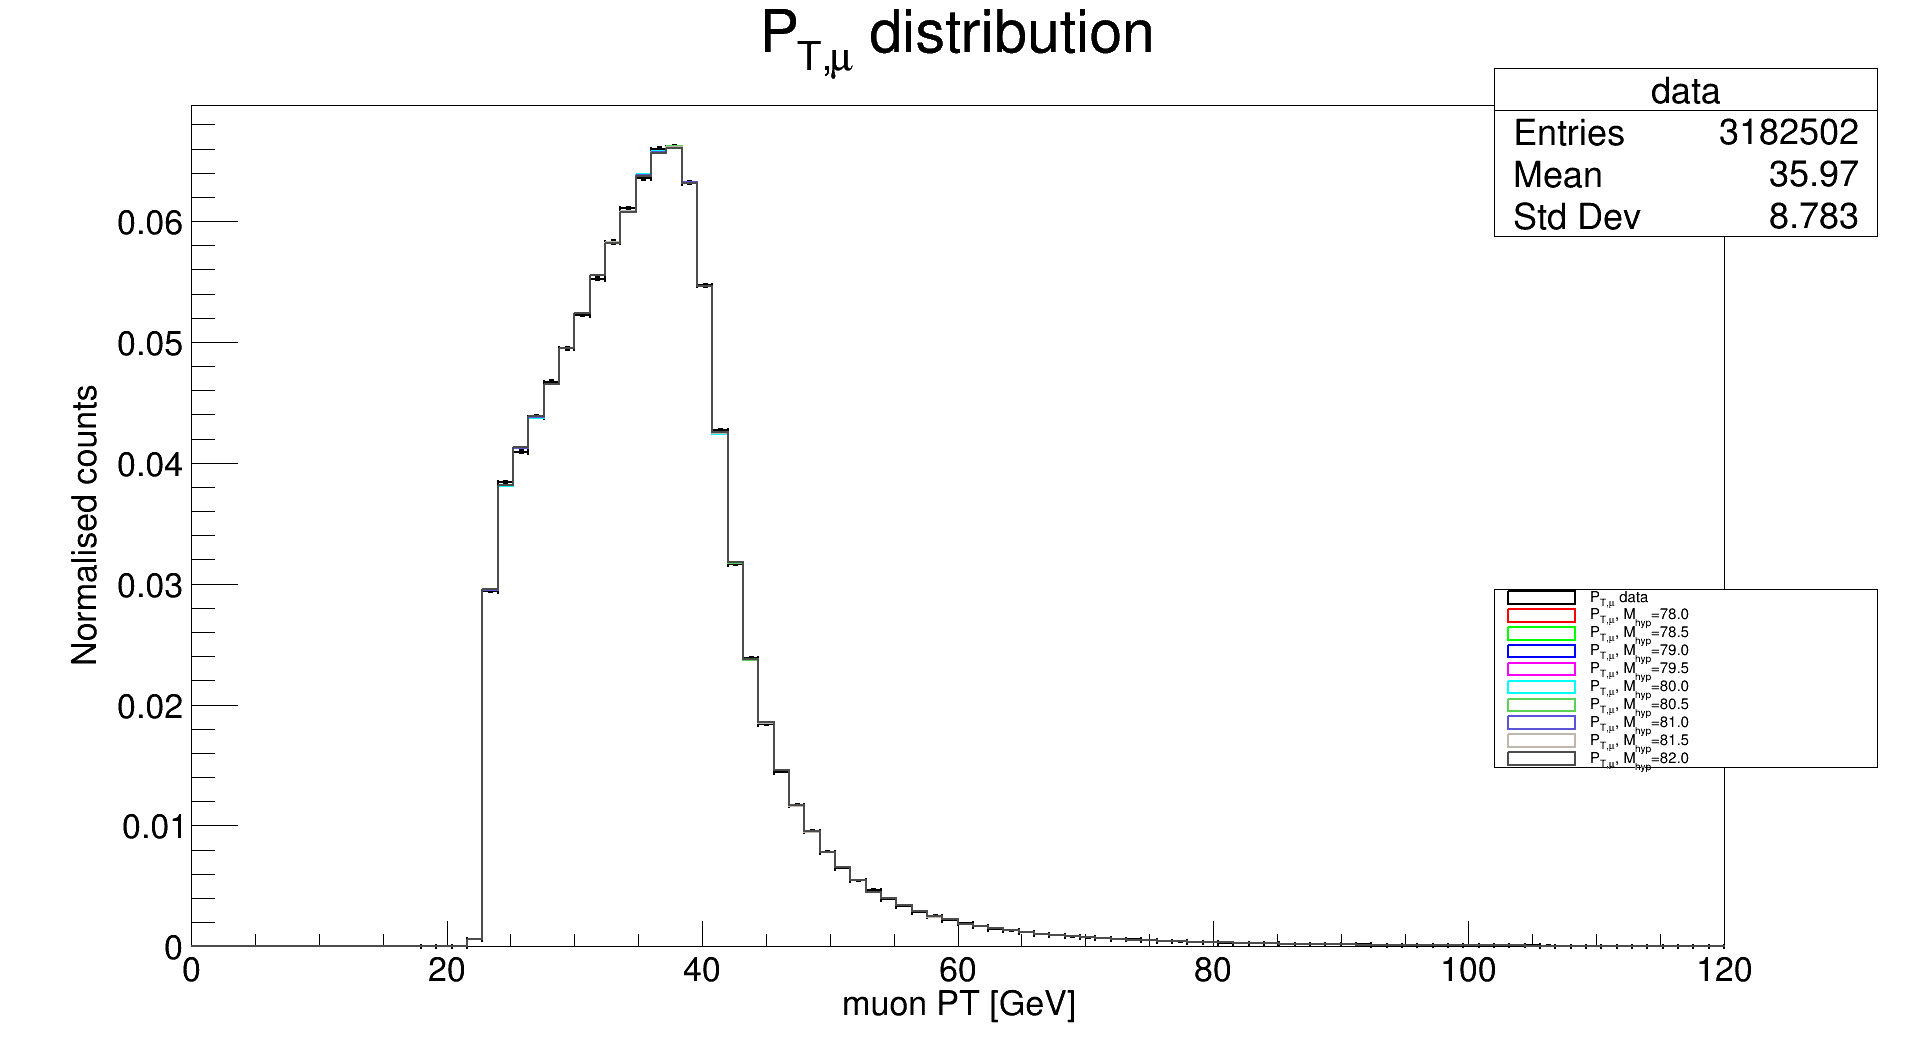
\includegraphics[width=\columnwidth]{/home/physics/phuxdp/Desktop/PX402 Physics Project/WBosonProject/T2W5/plots/muPT_80.379_2.07_between_78_and_82_summary.png}
		\caption{\small Hypothesis masses mean expected W mass: 80.379 $[GeV/c^{2}]$,\\
mean hypothesis masses: [78.  78.5 79.  79.5 80.  80.5 81.  81.5 82. ] $[GeV/c^{2}]$,\\
mass width: 2.07 $[GeV/c^{2}]$,\\
chi_square value of hypothesis fit: 54.120364976521856. }
		\label{fig: fig_0}
	\end{figure}

       \begin{figure}[tb]
		\centering
		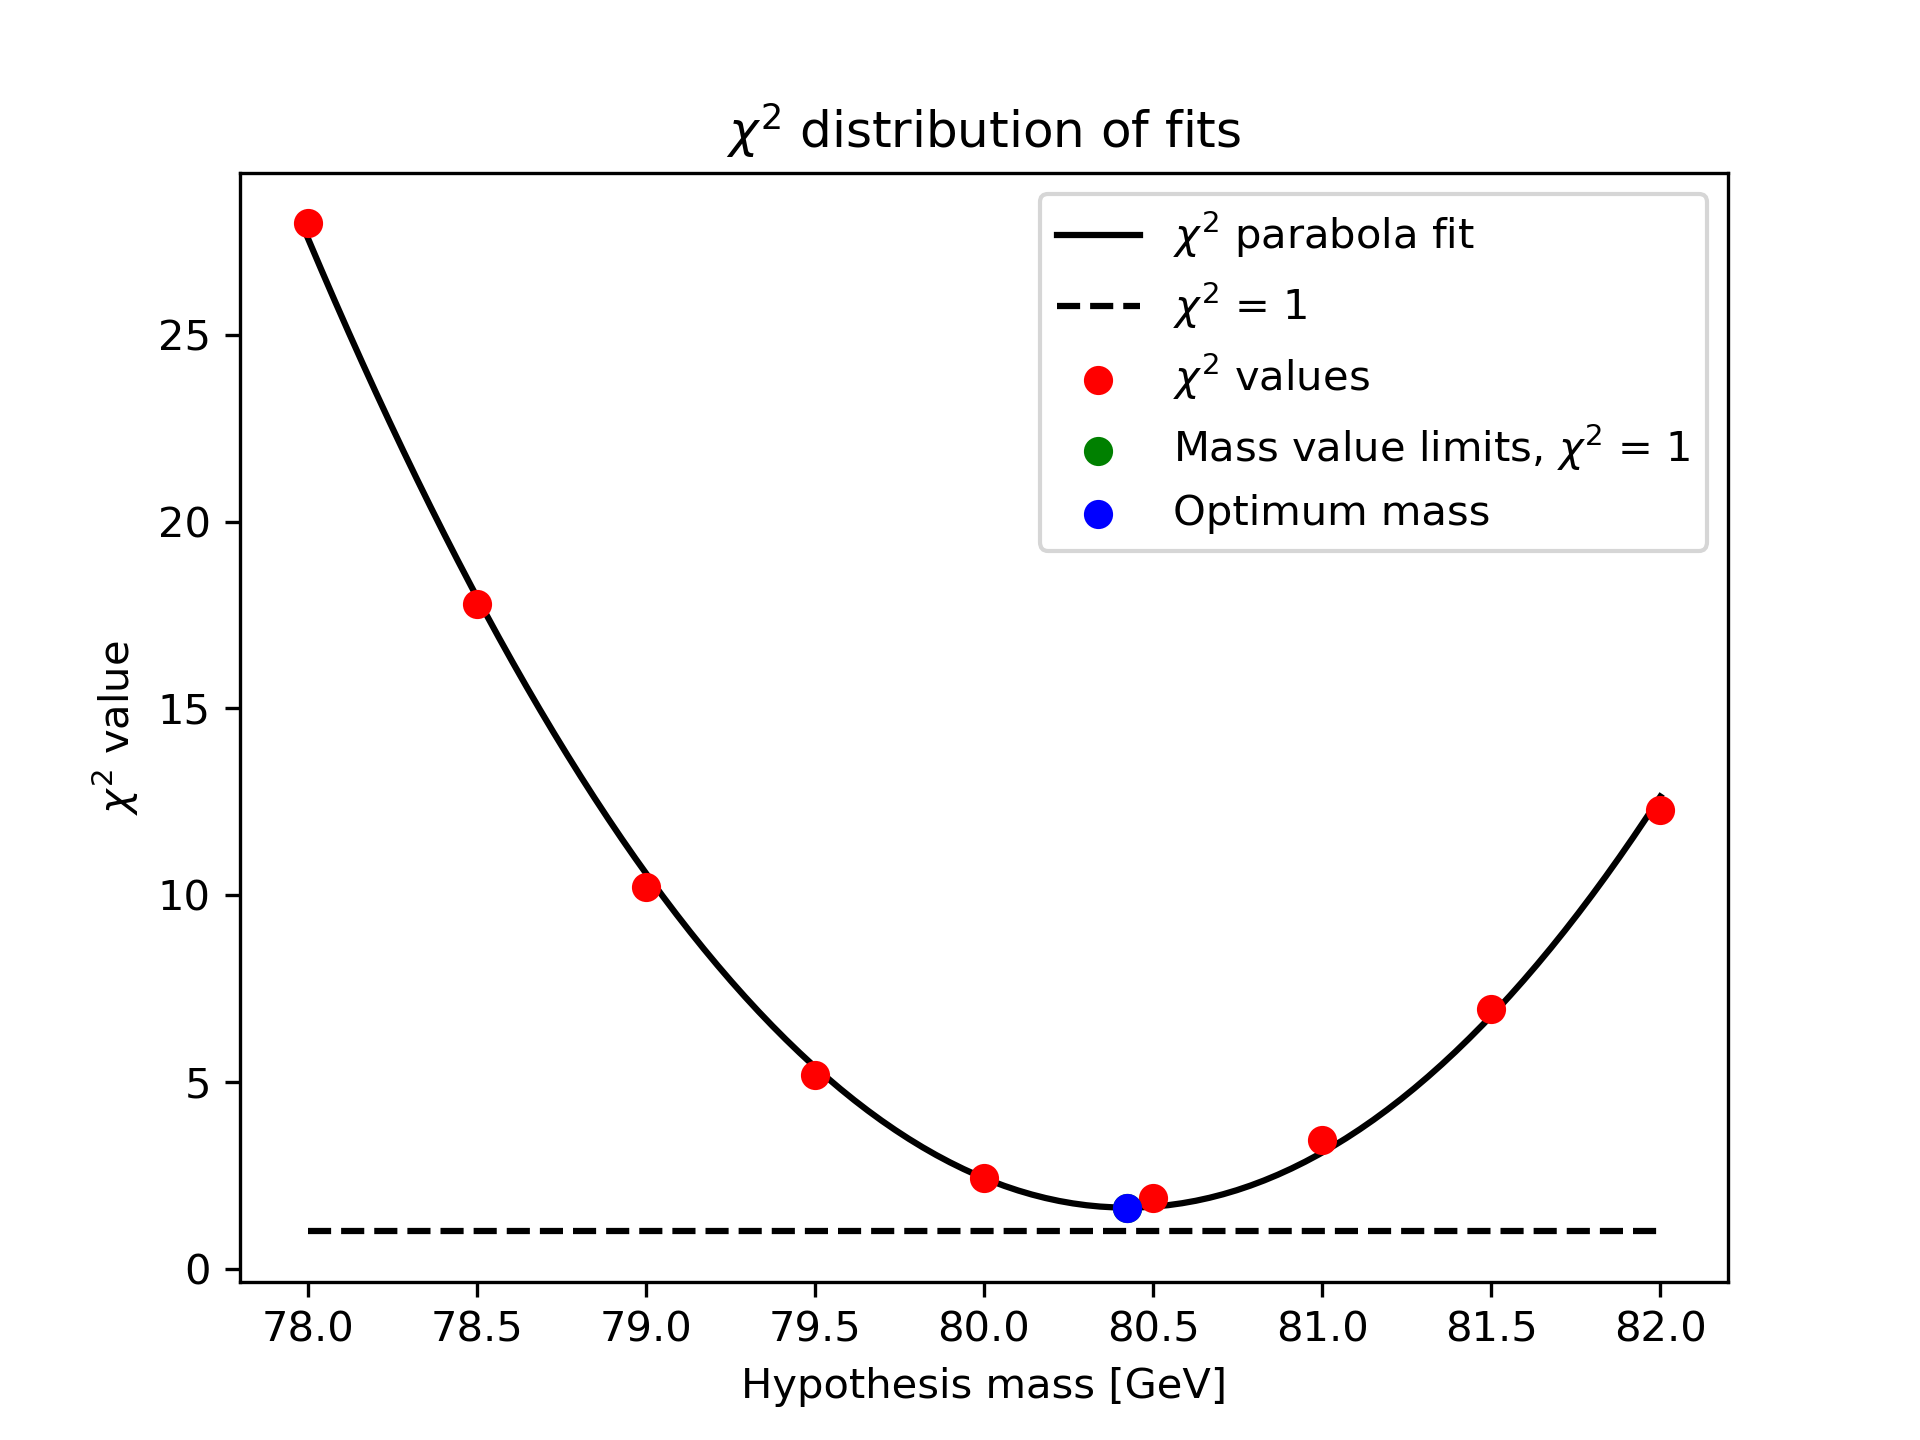
\includegraphics[width=\columnwidth]{/home/physics/phuxdp/Desktop/PX402 Physics Project/WBosonProject/T2W5/plots/chi_square_fits_muPT_80.379_2.07_between_78_and_82_summary.png}
		\caption{\small $\chi^2$ of hypothesis masses. }
		\label{fig: fig_chi_square}
	\end{figure}

    \begin{figure}[tb]
		\centering
		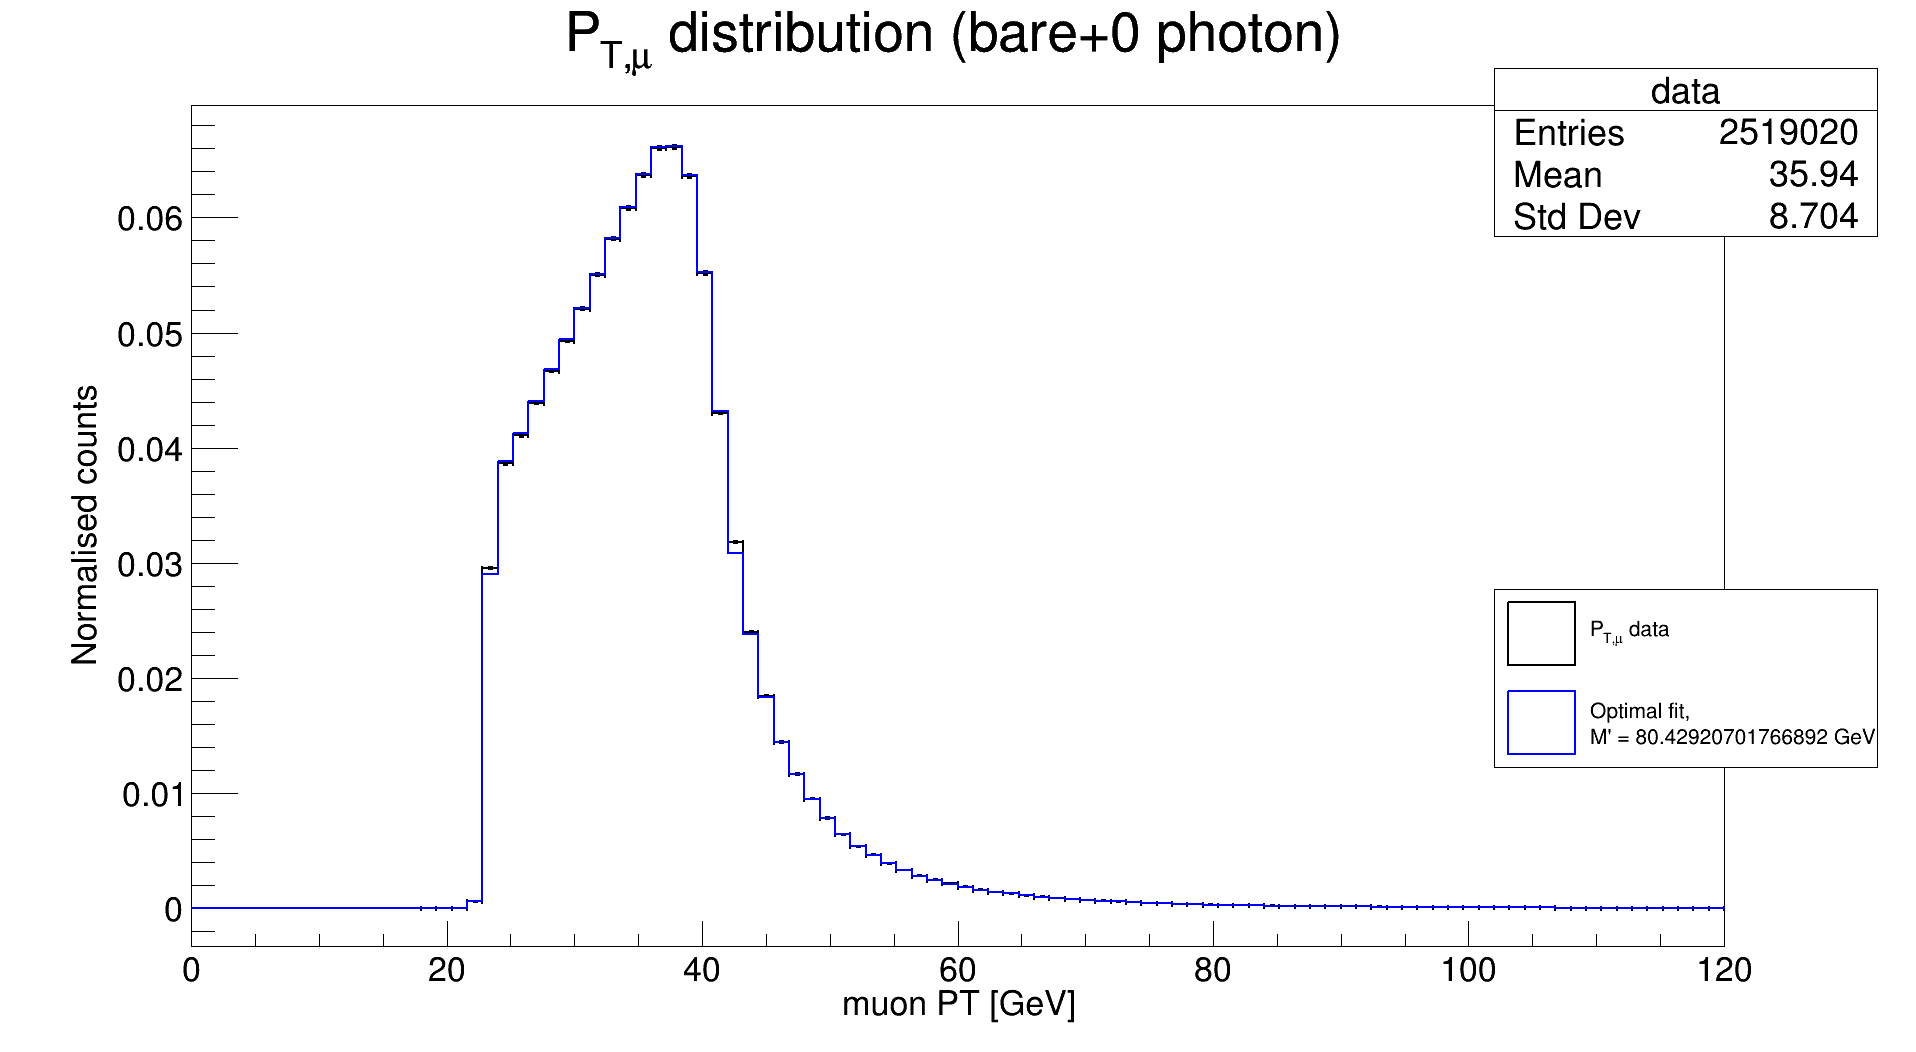
\includegraphics[width=\columnwidth]{/home/physics/phuxdp/Desktop/PX402 Physics Project/WBosonProject/T2W5/plots/optimum_muPT_80.379_2.07_between_78_and_82_summary.png}
		\caption{\small Data and optimum fit with $\chi^2 = 0.19001940879872306$. Used the hypothesis mass of 80.41009319280822$\pm$0.17501396541508996 $[GeV/c^{2}]$. }
		\label{fig: fig_optim_parms}
	\end{figure}
    
\end{document}